\chapter{Results and Discussion}

We have reviewed the rich history of hadronic spin physics and
identified the need to more precisely constrain the polarized gluon
distribution. We described the experimental apparatus and the analysis
techniques used to collect and study millions of polarized proton collisions
towards that end. This chapter presents the final results of the analysis, a set
of asymmetries that are directly sensitive to polarized glue and allow a deeper
understanding of the fundamental nature of QCD in the nucleon.

\section{$A_{LL}$ for Inclusive Charged Pion Production}

Figure~\ref{fig:final-result-run5} presents the first measurement of \(A_{LL}\)
for inclusive charged pion production at the STAR experiment. The data are
plotted versus the \(p_T\) of the pion and are compared to a variety of NLO pQCD
predictions. The dashed black curve represents a prediction for \(A_{LL}\) based
on the GRSV Standard parameterization of \(\Delta g(x)\), which was derived in
2001 from a global fit to polarized DIS data. The MIN and ZERO curves correspond
respectively to maximally negative and zero gluon polarization in the nucleon.
Not shown is the fourth member of the GRSV set, corresponding to maximal gluon
polarization, which has been excluded by earlier measurements of \(A_{LL}\) in
other final-state channels (and is similarly excluded by this measurement).

The dashed magenta curve labeled GS Set C is based on a polarized gluon
distribution by Gehrmann and Stirling that has a small integral polarization in
the \(x\) range accessible to 200 GeV mid-rapidity measurements at RHIC, but in
fact has a very large polarization content at smaller values of \(x\). Future
correlation measurements and measurements at a 500 GeV center-of-mass energy
will enable STAR to test whether distribution functions of this form might
correspond to reality. Finally, the solid black curve represents a new
parameterization of \(\Delta g(x)\) by de Florian, Sassot, Stratmann, and
Vogelsang which is based on a global fit incorporating both DIS data and early
\(A_{LL}\) results from RHIC.\footnote{The measurements in this thesis are not
included in the current DSSV global fit.}

\begin{figure}[ht]
  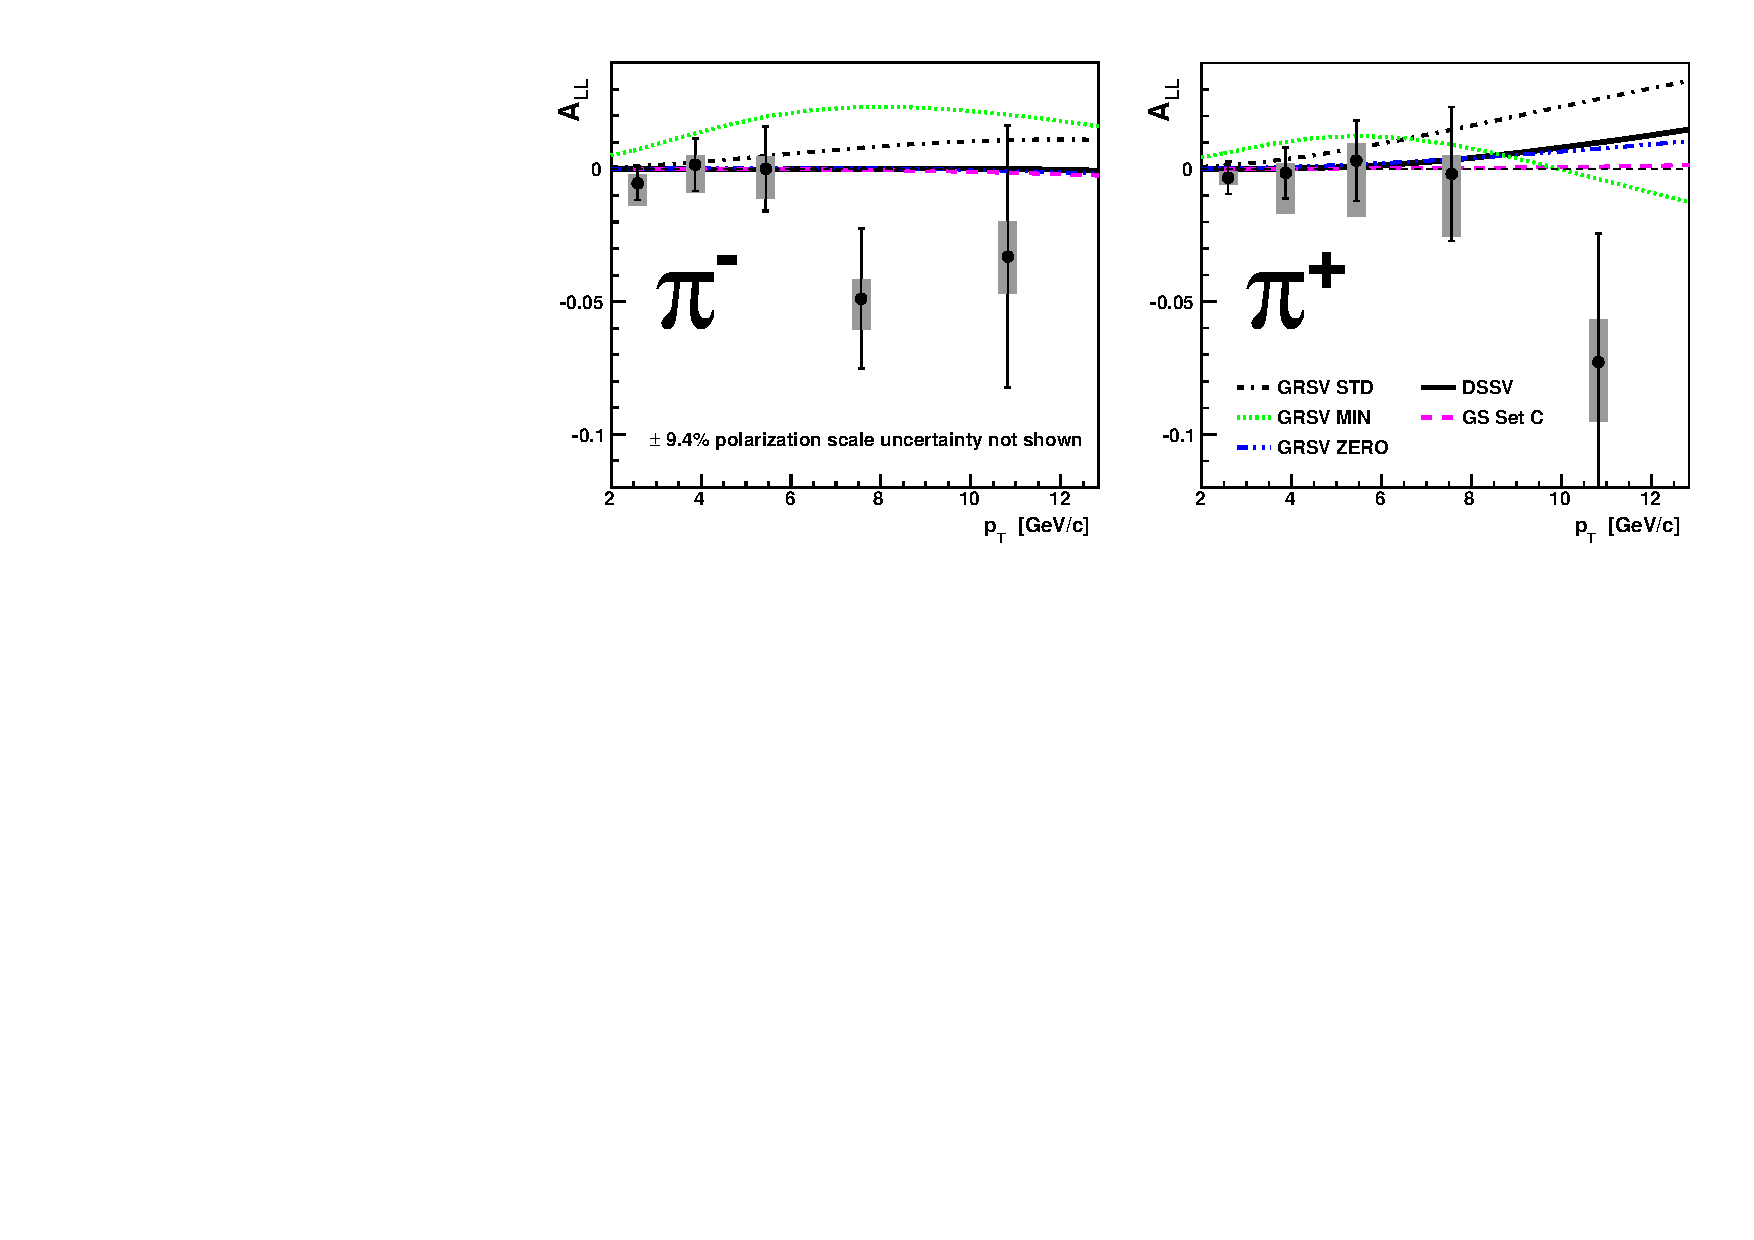
\includegraphics[width=1.0\textwidth]{figures/final-result-run5-2}
  \caption{$A_{LL}$ for inclusive charged pion production as a function of pion $p_T$ obtained from the 2005 dataset.  The error bars represent statistical uncertainties while the gray bands display total point-to-point systematic uncertainties.  The data are compared to NLO pQCD predictions incorporating various models for $\Delta g(x)$ \cite{Gluck:2000dy, Gehrmann:1995ag, deFlorian:2008mr}.}
  \label{fig:final-result-run5}
\end{figure}

\section{$A_{LL}$ for Jet + Pion Correlations}

Shown in Figure~\ref{fig:final-result-run6} are STAR's first measurements of
\(A_{LL}\) for charged pions opposite a trigger jet. The data are plotted versus
the fragmentation variable \(z\), using the away-side trigger jet \(p_T\) as a
surrogate for the \(p_T\) of the parton from which the pion fragmented. NLO pQCD
predictions for the measurement are plotted assuming the GRSV Standard, GS Set
C, and DSSV gluon distributions discussed above. The large difference in the
predictions for \(\pi^-\) \(A_{LL}\) and \(\pi^+\) \(A_{LL}\) at high \(z\) is a
reflection of the importance of favored fragmentation in that regime. Recall
that the \(\Delta u(x)\) distribution in the proton is uniformly positive, while
the \(\Delta d(x)\) distribution is smaller and uniformly negative. At high
\(z\), where the disparity between favored and disfavored fragmentation is
large, the \(\pi^-\) \(A_{LL}\) is driven by \(d\) quark scattering and the
\(\pi^+\) by \(u\) quark scattering. Favored fragmentation is also responsible
for the very different functional forms of the MIN \(A_{LL}\) prediction for
inclusive \(\pi^-\) and \(\pi^+\) \(A_{LL}\) in
Figure~\ref{fig:final-result-run5}.

\begin{figure}[]
  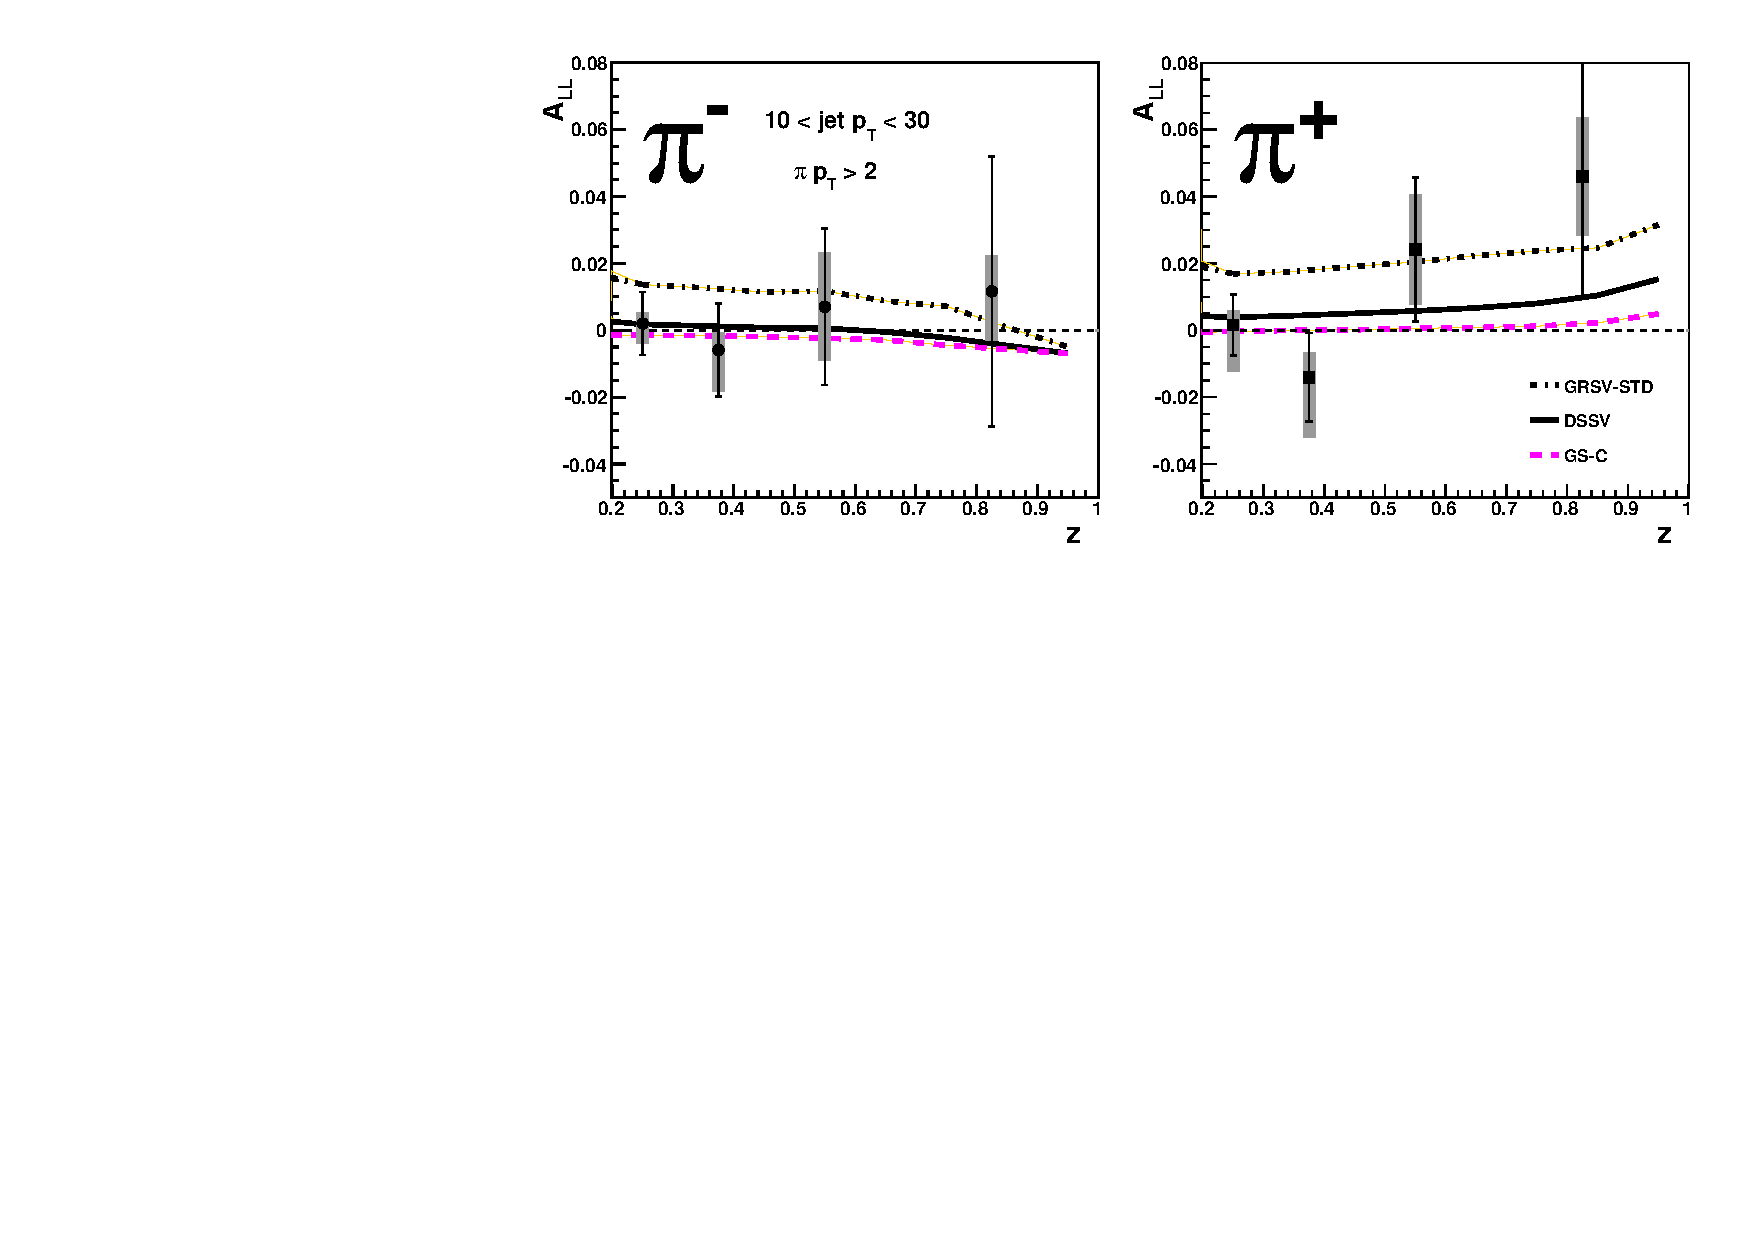
\includegraphics[width=1.0\textwidth]{figures/final-result-run6-4}
  \caption{$A_{LL}$ for charged pion production opposite an identified jet from the 2006 dataset.  The data are plotted against the ratio of the pion and jet transverse momenta, here labeled using the fragmentation variable $z$.  As in Figure~\ref{fig:final-result-run5}, the error bars represent statistical uncertainties and the gray bands point-to-point systematics.  The NLO predictions are the result of a recent analysis by de Florian \cite{deFlorian:2009fw}.}
  \label{fig:final-result-run6}
\end{figure}

\begin{table}
  \centering
  \begin{tabular}{|c||c|c|c||c|c|c|}
    \hline
    \multirow{2}{*}{$p_T$} & \multicolumn{3}{c||}{$\pi^{-}$} & \multicolumn{3}{c|}{$\pi^{+}$} \\
    \cline{2-7}
    & $A_{LL}$ & Stat. Error & Syst. Error &$A_{LL}$ & Stat. Error & Syst. Error\\
    (GeV/c) & ($10^{-3}$) & ($10^{-3}$) & ($10^{-3}$) & ($10^{-3}$) & ($10^{-3}$) & ($10^{-3}$) \\
    \hline
    \hline
    2.00 - 3.18 & -5.5 & $\pm$ 6.3 & -8.2 +3.4 &  -3.3 & $\pm$ 6.1 & -2.7 +2.2\\
    3.18 - 4.56 & 1.6 & $\pm$ 9.9 & -10.4 +3.4 &  -1.5 & $\pm$ 9.5 & -15.2 +3.5\\
    4.56 - 6.32 & 0.0 & $\pm$ 15.9 & -11.2 +4.6 &  3.1 & $\pm$ 15.2 & -21.1 +6.5\\
    6.32 - 8.80 & -48.9 & $\pm$ 26.4 & -11.4 +7.3 &  -1.9 & $\pm$ 25.2 & -23.5 +7.1\\
    8.80 - 12.84 & -33.0 & $\pm$ 49.4 & -14.0 +13.2 &  -72.8 & $\pm$ 48.5 & -22.2 +16.0\\
    \hline
  \end{tabular}
  \caption{$A_{LL}$ for inclusive charged pion production.}
  \label{tab:final-2005-result}
\end{table}

\begin{table}
  \centering
  \begin{tabular}{|c||c|c|c||c|c|c|}
    \hline
    \multirow{3}{*}{$z$} & \multicolumn{3}{c||}{$\pi^{-}$} & \multicolumn{3}{c|}{$\pi^{+}$} \\
    \cline{2-7}
    & $A_{LL}$ & Stat. Error & Syst. Error &$A_{LL}$ & Stat. Error & Syst. Error\\
    & ($10^{-3}$) & ($10^{-3}$) & ($10^{-3}$) & ($10^{-3}$) & ($10^{-3}$) & ($10^{-3}$) \\
    \hline
    \hline
    0.20 - 0.30 & 2.0 & $\pm$ 9.4 & -6.1 +3.2 &  1.6 & $\pm$ 9.1 & -14.0 +4.2\\
    0.30 - 0.45 & -5.9 & $\pm$ 13.9 & -12.4 +5.2 &  -14.1 & $\pm$ 13.2 & -18.0 +7.4\\
    0.45 - 0.65 & 7.0 & $\pm$ 23.4 & -16.1 +16.1 &  24.1 & $\pm$ 21.5 & -16.3 +16.5\\
    0.65 - 1.00 & 11.6 & $\pm$ 40.4 & -14.8 +10.6 &  46.0 & $\pm$ 36.5 & -17.7 +17.7\\
    \hline
  \end{tabular}
  \caption{$A_{LL}$ for charged pions opposite a trigger jet.}
  \label{tab:final-2006-result}
\end{table}

\section{Interpretation and Future Work}

A quantitive comparison of a measurement and an associated NLO prediction is obtained by calculating the \(\chi^2\) of the measurement with respect to the prediction.  One can then report the confidence level for that model of the polarized gluon distribution, which represents the probability that a \(\chi^2\) would exceed the observed \(\hat{\chi}^2\) if the model is correct.  Table~\ref{tab:confidence-levels} lists the confidence levels for all theoretical predictions plotted in Figures~\ref{fig:final-result-run5} and \ref{fig:final-result-run6}.  The \(\chi^2\) statistics are computed using statistical and point-to-point systematic uncertainties summed in quadrature.

The data are clearly incompatible with an assumption of maximally polarized gluons.  Maximally negative gluon polarization is also excluded at the 97.9\% level.  In general, the data are consistent with previous RHIC measurements in their preference for small values of gluon polarization.

The experimental methods described in this thesis are equally applicable to recent and future data taking at STAR.  A better understanding of systematic uncertainties in measurements of charged pion \(A_{LL}\) can be obtained through detailed Monte Carlo simulations of pion fragmentation as well as tighter constraints on the jet transverse momentum scale uncertainty.  Increases in luminosity and  polarization, as well as the first collisions at \(\sqrt{s} = 500\) GeV, speak to a bright future for RHIC as the experiments continue a comprehensive investigation into the spin structure of the nucleon.

\begin{table}
  \centering
  \begin{tabular}{|l||c|c|c|c|}
    \hline
    \multirow{2}{*}{Gluon Polarization Scenario} & \multicolumn{4}{c|}{Confidence Level} \\
    \cline{2-5}
    & 2005 $\pi^-$ & 2005 $\pi^+$ & 2006 $\pi^-$ & 2006 $\pi^+$ \\
    \hline
    GRSV $\Delta g$ = g & 1.6e-06 & 2e-07 & - & - \\
    GRSV $\Delta g$ = -g & 0.016 & 0.32 & - & - \\
    GRSV $\Delta g$ = 0 & 0.52 & 0.72 & - & - \\
    GRSV STD & 0.31 & 0.41 & 0.56 & 0.13 \\
    GS Set C & 0.53 & 0.79 & 0.98 & 0.59 \\
    DSSV & 0.52 & 0.71 & 0.98 & 0.59 \\
    \hline
  \end{tabular}
  \caption{Confidence levels of fitting predictions for $A_{LL}$ based on various polarized gluon distributions to the measurements presented in this thesis.}
  \label{tab:confidence-levels}
\end{table}
